\documentclass[11pt,compress,t,notes=noshow, aspectratio=169, xcolor=table]{beamer}

\usepackage{../../style/lmu-lecture}
% Defines macros and environments
% This file is included in slides and exercises

% Rarely used fontstyle for R packages, used only in 
% - forests/slides-forests-benchmark.tex
% - exercises/single-exercises/methods_l_1.Rnw
% - slides/cart/attic/slides_extra_trees.Rnw
\newcommand{\pkg}[1]{{\fontseries{b}\selectfont #1}}

% Spacing helpers, used often (mostly in exercises for \dlz)
\newcommand{\lz}{\vspace{0.5cm}} % vertical space (used often in slides)
\newcommand{\dlz}{\vspace{1cm}}  % double vertical space (used often in exercises, never in slides)
\newcommand{\oneliner}[1] % Oneliner for important statements, used e.g. in iml, algods
{\begin{block}{}\begin{center}\begin{Large}#1\end{Large}\end{center}\end{block}}

% Don't know if this is used or needed, remove?
% textcolor that works in mathmode
% https://tex.stackexchange.com/a/261480
% Used e.g. in forests/slides-forests-bagging.tex
% [...] \textcolor{blue}{\tfrac{1}{M}\sum^M_{m} [...]
% \makeatletter
% \renewcommand*{\@textcolor}[3]{%
%   \protect\leavevmode
%   \begingroup
%     \color#1{#2}#3%
%   \endgroup
% }
% \makeatother


\title{Applied Machine Learning}
% \author{LMU}
%\institute{\href{https://compstat-lmu.github.io/lecture_iml/}{compstat-lmu.github.io/lecture\_iml}}
\date{}

\begin{document}

\begin{frame}{Lift Charts}

\begin{itemize}
\setlength\itemsep{1em}
    \item Lift charts visualize a model's ability to detect events.
    \item Samples are ranked according to their scores (probability for an event to take place). We then evaluate the cumulative event rate.
    \item In the optimal case, we would suspect the $m$ highest ranked samples to contain all $m$ events.
    \item For a non-informative model, the fraction $\frac{k}{n}$ of the highest ranked samples contains $k$ events on average.
    \item For a more informative model, the fraction $\frac{k}{n}$ of the highest ranked samples contains more than $k$ events.
    \item The \textbf{lift} corresponds to the amount of events detected by a model above a completely random selection of samples.
\end{itemize}
\end{frame}



\begin{frame}{Lift Chart Example}
\begin{columns}
\begin{column}{0.5\textwidth}
\begin{itemize}
    \item We plot the cumulative event rate against the percentage of screened observations.
    \item Here, we face a 50\% event rate. For a perfect model, the 50\% highest ranked observations contain 50\% of all events.
    \item We create a lift curve for a non-informative model which runs along the diagonal line.
    \item Another model is able to perfectly detect events. After evaluating 50\% of the observations associated with the highest event probabilities, we have captured all events.
\end{itemize}
\end{column}
\begin{column}{0.5\textwidth}
\begin{figure}
    \centering
    \includegraphics[width = \textwidth]{figure/lift_chart.png}
    \caption{Lift chart from Applied Predictive Modeling (Max Kuhn).}
\end{figure}
\end{column}

\end{columns}

\end{frame}


% \begin{frame}{Pseudo Code to Create Lift Chart}

% To construct a lift chart, we follow a general recipe:
% \begin{itemize}
% \setlength\itemsep{2em}
%     \item Predict target values for a sample that was not used during training with known target values.
%     \item Compute fraction of true events in the
% entire data set (= baseline event rate).
%     \item Rank data by scores (probability of event taking place).
%     \item For every unique event probability $\phi$, compute: 
%     $$\frac{\text{percentage of events in all observations with scores below $\phi$}}{\text{baseline event rate}}$$
% \end{itemize}
% \end{frame}

\begin{frame}{Calibration Curves}

\begin{columns}

\begin{column}{0.5\textwidth}
\begin{itemize}
\setlength\itemsep{2em}
    \item Calibration curves plot the true frequency of the positive label against its predicted probability for binned predictions.
    \item The horizontal axis represents the average predicted probability in each bin. The vertical axis indicates the the proportion of predicted positive labels.
    \item A well-calibrated classifier is associated with a diagonal clibration curve.
\end{itemize}
\end{column}
\begin{column}{0.5\textwidth}
\begin{figure}
    \centering
    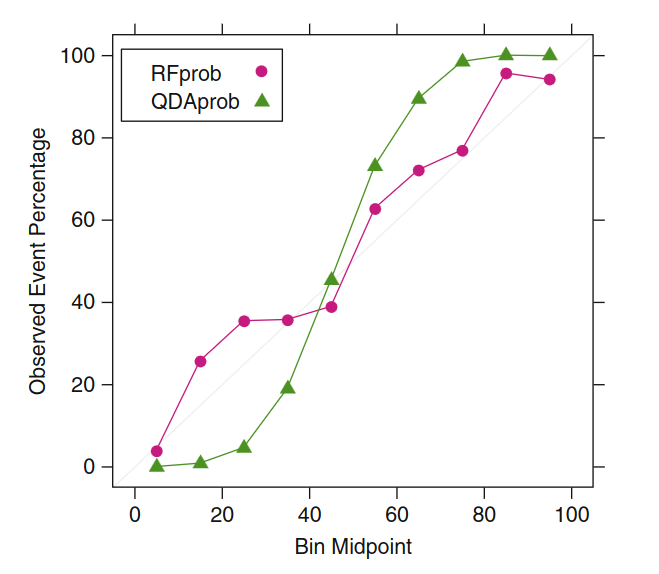
\includegraphics{figure/calibration_plot.png}
    \caption{Calibration plot from Applied Predictive Modeling (Max Kuhn).}
\end{figure}
\end{column}
\end{columns}

\end{frame}



\endlecture
\end{document}
